\chapter{Implementazione Software: Design del Protocollo}
\label{chap:implementazione_software}

\section{Architettura generale del sistema}

Il software è stato sviluppato in linguaggio \textbf{C}. 
Questa scelta permette di avere un controllo diretto sull’hardware dell’ESP32,
 ottenendo esecuzioni prevedibili ed un uso minuzioso delle risorse. \\
 L’utilizzo del C ha inoltre garantito maggiore leggerezza rispetto al C++ e una buona portabilità, grazie alla disponibilità di librerie 
 già consolidate in ambito firmware.  

Alcune librerie Arduino originariamente scritte in C++ sono state adattate in C questo per permettere la compilazione del codice.\\
 Allo stesso tempo, l’uso del framework Arduino su 
  ESP32 ha offerto vantaggi importanti tra cui: documentazione estesa, supporto diretto alle periferiche del microcontrollore e una 
  community ampia, che ha velocizzato la fase di sviluppo. \\

Per lo sviluppo è stato utilizzato \textit{Visual Studio Code}, scelto per l’ampia disponibilità di estensioni.
 In particolare, l’integrazione con \textbf{PlatformIO} ha reso più semplice la gestione del progetto: compilazione, caricamento e debugging sono stati 
 unificati in un unico ambiente, con gestione automatica delle librerie e delle dipendenze, ha permesso uno sviluppo più rapido ed organizzato.\\ 

L’architettura complessiva si basa su moduli separati e specializzati, ognuno responsabile di una parte precisa del protocollo. 
Questo approccio modulare ha garantito una migliore manutenibilità del codice e ha semplificato l’integrazione tra i diversi livelli funzionali 
descritti in \autoref{chap:design_protocollo}.

\section{Emissione dei toni}

L’uscita audio discussa nella \autoref{sec:uscita_livello_fisico} è gestita dal modulo \textbf{audio\_driver}, 
responsabile dell’inizializzazione del bus I\textsuperscript{2}S e della generazione in tempo reale delle sinusoidi che rappresentano i bit. \\
La funzione \textbf{play\_two\_tones} produce due toni simultanei, richiedendo come parametri le due frequenze delle quali dovrà generare le sinusoidi.
La generazione del segnale avviene con persistenza di fase, evitando discontinuità tra un’emissione e la successiva. 


\begin{minted}[linenos,breaklines]{c}
void play_two_tones(int freq1, int freq2) {
    if(freq1 == 0 && freq2 == 0){
        delay(80);
    } else {
        const float tone_duration = 0.024f;
        const int tone_samples = (int)(G_SAMPLE_RATE * tone_duration);
        const int tone_buffer_size = tone_samples * 2;
        int16_t tone_buffer[tone_buffer_size];
    \end{minted}
Le variabili sotto garantiscono la continuità di fase tra chiamate successive della funzione:
\begin{minted}[linenos,breaklines]{c}
        static float phase1 = 0.0f;
        static float phase2 = 0.0f;
        const float inc1 = 2.0f * PI * freq1 / G_SAMPLE_RATE;
        const float inc2 = 2.0f * PI * freq2 / G_SAMPLE_RATE;
    \end{minted}
Questo frammento di codice mostra la generazione del buffer di campioni,
 che viene poi scritto sul bus I\textsuperscript{2}S:
\begin{minted}[linenos,breaklines]{c}
        for (int i = 0; i < tone_samples; i++) {
            float mixed = sinf(phase1) + sinf(phase2);
            int16_t sample = (int16_t)(3000 * (mixed / 2.0f));
            tone_buffer[2 * i] = sample;
            tone_buffer[2 * i + 1] = sample;
            phase1 += inc1;
            if (phase1 >= 2.0f * PI) phase1 -= 2.0f * PI;
            phase2 += inc2;
            if (phase2 >= 2.0f * PI) phase2 -= 2.0f * PI;
        }
        size_t bytes_written = 0;
        i2s_write(I2S_NUM, tone_buffer, sizeof(tone_buffer), &bytes_written, portMAX_DELAY);
    }
}
\end{minted}

L’ampiezza massima del segnale è limitata a un valore inferiore a 32767 per evitare saturazioni sul DAC, questa conclusione deriva
 da test che hanno mostrato come 
 il fattore di scaling a \textbf{3000} garantisce \textbf{headroom sufficiente}. Quando entrambe le frequenze sono nulle,
  la routine introduce una pausa di \textbf{80 ms}, che equivale a una “inattività” progettata per separare gruppi di
   simboli o pacchetti.

\section{Campionamento e bufferizzazione}

Il percorso inverso, ovvero l’acquisizione dei toni ricevuti, discusso nella \autoref{sec:ingresso_livello_fisico} come l'ingresso del Livello Fisico 
è affidato al \textbf{reader}.  \\ 
Il modulo crea due buffer circolari tra cui effettua un meccanismo di \textbf{swapping sincronizzato}: mentre uno viene riempito dal task di I\textsuperscript{2}S, 
l’altro è disponibile per l’elaborazione FFT, questo avviene attraverso un insieme di variabili rese \textbf{extern} e mediante l'uso di un \textbf{puntatore} 
con attributo \textbf{extern} che punta sempre al buffer pronto, cosi da renderlo disponibile alla funzione richiedente senza che questa entri nella 
logica del reader. \\

\begin{minted}[linenos,breaklines]{c}
extern volatile int data_ready;
extern volatile int status_flag;
extern complex_g3_t *array_ready;
\end{minted}

La funzione \textbf{reader\_task} legge i campioni dal bus I\textsuperscript{2}S, li converte in numeri complessi e li memorizza nel buffer corrente.\\

\begin{minted}[linenos,breaklines]{c}
static void reader_task(void *param) {
    size_t bytes_read;
    int32_t dma_buffer[DMA_BUFFER_SIZE / 4];
    static float dc_mean = 0.0f;
    const float alpha = 1.0f / 1024.0f;
    while (1) {
        i2s_read(I2S_PORT, (void*)dma_buffer, DMA_BUFFER_SIZE, &bytes_read, portMAX_DELAY);
        int samples = bytes_read / 4;
        for (int i = 0; i < samples; i++) {
            int32_t s32 = dma_buffer[i] >> 8;
            float x = (float)(s32 >> 12);
            dc_mean += alpha * (x - dc_mean);
            float val = x - dc_mean;
            current_data[counter].re = (double)val;
            current_data[counter].im = 0.0;
            counter++;
            if (counter >= ARRAY_ELEMENTS) {
                data_ready = 1;
                swap_array();
                counter = 0;
            }
        }
    }
}
\end{minted}

L’eliminazione della componente DC avviene con una media mobile parametrizzata da \textbf{alpha}, \\ 
il quale viene; i campioni centrati vengono convertiti in numeri complessi con parte immaginaria nulla per l’elaborazione spettrale.\\
L’uso di \textbf{swap\_array} consente di non perdere alcun campione e di garantire un’elaborazione a flusso continuo.  \\

\begin{minted}[linenos,breaklines]{c}
 static void swap_array(void) {
     array_ready = current_data;
     current_data = (current_data == main_array) ? secondary_array : main_array;
 }
 \end{minted}

\begin{figure}[H]
    \centering
    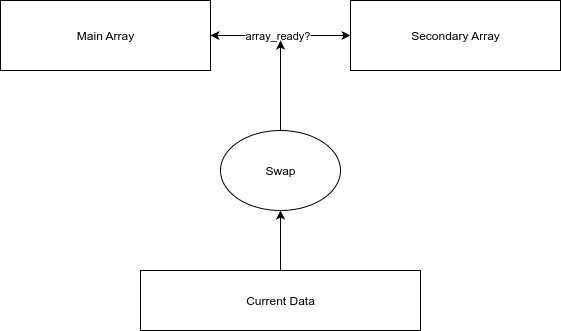
\includegraphics[width=0.6\textwidth]{immagini/swapping_array.png}
    \caption{Swapping degli array di campioni}
    \label{fig:swapping_array}
\end{figure}

\section{Trasformata veloce di Fourier}
Altro aspetto critico del Livello Fisico è la trasformata rapida di Fourier (FFT), che converte i campioni temporali in rappresentazioni spettrali. 
Cosi come discusso nella \autoref{par: fft_calcolo}, l’implementazione adottata è una versione personalizzata dell’algoritmo di Cooley–Tukey, ottimizzata per
 il contesto real-time e per la risoluzione richiesta. \\
 L'analisi frequenziale viene eseguita nel modulo \textbf{fft.c}, questa include due funzioni principali \textbf{FFT\_get\_twiddle\_factors} e \textbf{FFT\_calculate}. \\

\begin{minted}[linenos,breaklines]{c}
void FFT_calculate (complex_g3_t *x, long N, complex_g3_t *X,
                    complex_g3_t *scratch, complex_g3_t *twiddles){
    int k, m, n;
    int skip;
    boolean evenIteration = N & 0x55555555;
    complex_g3_t* E;
    complex_g3_t* Xp, *Xp2, *Xstart;
    if (N == 1){
        X[0] = x[0];
        return;
    }
    E = x;
    for (n = 1; n < N; n = n * 2){
        Xstart = evenIteration ? scratch : X;
        skip = N / (2 * n);
        Xp = Xstart;
        Xp2 = Xstart + N / 2;
        for (k = 0; k < n; k++){
            double tim = twiddles[k * skip].im;
            double tre = twiddles[k * skip].re;
            for (m = 0; m < skip; ++m){
                complex_g3_t* D = E + skip;
                double dre = D->re * tre - D->im * tim;
                double dim = D->re * tim + D->im * tre;
                Xp->re  = E->re + dre;
                Xp->im  = E->im + dim;
                Xp2->re = E->re - dre;
                Xp2->im = E->im - dim;
                ++Xp; ++Xp2; ++E;
            }
            E += skip;
        }
        E = Xstart;
        evenIteration = !evenIteration;
    }
}
\end{minted}

Lo schema fa uso di array globali per l’uscita e per lo spazio temporaneo, così da evitare allocazioni
 dinamiche che in un contesto real-time sarebbero troppo costose.\\
  Il flag \textbf{evenIteration} serve 
 a gestire il ping-pong tra l’array risultato e quello di appoggio:
 in questo modo si alternano i ruoli dei due buffer a ogni passo, senza dover copiare dati inutilmente.


 \section{Decodifica spettrale}

 Le frequenze individuate dalla trasformata passano al modulo \textbf{decoder}, 
 che ha il compito di capire se un picco spettrale corrisponde davvero a un tono
  del protocollo oppure se si tratta di rumore. Questa logica è implementata nella funzione
   \textbf{check\_active\_frequencies}, che lavora in tre fasi: calcolo della soglia dinamica,
    controllo dei massimi locali e interpolazione del picco confermato.  
 
 \begin{minted}[linenos,breaklines]{c}
 struct_interpolated_frequency check_active_frequencies(
         complex_g3_t *data, int bin_1, int bin_2,
         int id, double noise_floor){
     int i, j;
     struct_interpolated_frequency detected_freq;
     detected_freq.work = 0;
     detected_freq.frequency = -1.0;
     detected_freq.estimated_amplitude = -1.0;
     detected_freq.dynamic_amplitude_threshold = -1.0;
 \end{minted}
 
 La funzione crea una struttura \textbf{detected\_freq} che conterrà il risultato. 
 Tutti i campi sono inizializzati a valori “non validi” (ad esempio -1.0) così che, 
 se nessuna frequenza viene trovata, il chiamante può accorgersene immediatamente.  
 
 \begin{minted}[linenos,firstnumber=14,breaklines]{c}
     for (j = bin_1; j <= bin_2; j++){
         double freq = (double)(FS * j) / NN;
         double amp = complex_magnitude(data[j]);
 \end{minted}
 
 Il ciclo scorre i bin tra \textbf{bin\_1} e \textbf{bin\_2} che, come discusso nel \autoref{subsec:filtraggio} i bin sono 
 la rappresentazione discreta della frequenza nello spettro ottenuto dalla FFT.
 \begin{equation}
    bin[i] = (FS * i) / NN = (48000 * i) / 512 = 93.75 * i.
 \end{equation}
  La formula calcola la frequenza corrispondente a ogni bin, dove \textbf{FS} è la frequenza di campionamento e \textbf{NN} il numero di punti della FFT.\\
  Il BIN è quindi un indice che rappresenta una specifica frequenza nell'array risultante dalla FFT.\\
   La funzione \textbf{complex\_magnitude} calcola il modulo del numero complesso associato al bin corrente, che rappresenta l’ampiezza del segnale a quella frequenza.\\

 \begin{minted}[linenos,firstnumber=18,breaklines]{c}
         if(G_LINEAR_REGRESSION_MODE == 0){
             double dynamic_amplitude_threshold = noise_floor * 8.0;
             if (amp > dynamic_amplitude_threshold){
                 for(i = j-6; i < j + 6 && complex_magnitude(data[i]) <= amp; i++) {}
                 if (i == j+6){
                     detected_freq = interpolate_peak_frequency(data, j, FS, NN);
                     detected_freq.dynamic_amplitude_threshold = dynamic_amplitude_threshold;
                     detected_freq.work = 1;
                     return detected_freq;
                 }
             }
 \end{minted}
 
La soglia dinamica (dynamic\_amplitude\_threshold) è otto volte il \textbf{noise\_floor}.
 Una volta superata la soglia, viene controllata una finestra di 12 bin, come rappresentato in \autoref{fig:bins_local_peak} (sei a sinistra e sei a destra) 
 per assicurarsi che il valore corrente sia davvero un massimo locale. \\
Solo in questo caso si invoca \textbf{interpolate\_peak\_frequency}, le quali motivazioni e funzionamento sono spiegate nel \autoref{par: interpolazione_parabolica},
 che con una formula di interpolazione parabolica calcola la frequenza “vera”, 
per sopperire alla bassa risoluzione spettrale, questa tecnica, quindi fornisce una precisione sub-bin, cioè di una frequenza intermedia tra due bin adiacenti.\\  

 
 Infine, se nessuna frequenza valida è trovata, la funzione ritorna la struttura con i valori -1.0.  
 
 \section{Traduzione frequenza-bit}
 
 Una volta isolati i picchi, i moduli riguardanti il Livello Fisico lasciano spazio ai \textbf{moduli del Livello Bit} il primo passo è tradurli in 
 \textbf{Signal Codes} come nella seguente tabella.
  Questa operazione è svolta dal modulo \textbf{bit\_freq\_codec}, e in particolare dalla funzione \textbf{interpret\_bits}.  

  \definecolor{lightgray}{RGB}{235,235,235}
\definecolor{white}{RGB}{255,255,255}


  \begin{table}[H]
    \centering
    \label{tab:freq_codici_divisi}
    \begin{tabular}{|l|>{\columncolor{lightgray}}l|>{\columncolor{lightgray}}l|}
    \hline
    \textbf{Frequenza} & \textbf{Signal Code (0)} & \textbf{Signal Code (1)} \\
    \hline
    1400 & (0) & \\
    1800 & (1) & \\
    2200 & (2) & \\
    2600 & (3) & \\
    3000 & (4) & \\
    3400 & (5) & \\
    3800 & (6) & \\
    4200 & (7) & \\
    4600 & (8) & \\
    5000 & & (9) \\
    5400 & & (10) \\
    5800 & & (11) \\
    6200 & & (12) \\
    6600 & & (13) \\
    7000 & & (14) \\
    7400 & & (15) \\
    7800 & & (16) \\
    8200 & & (17) \\
    \hline
    \end{tabular}
    \caption{Mappatura frequenze con divisione dei Signal Code in 0 e 1}
\end{table}



 \begin{minted}[linenos,breaklines]{c}
 int interpret_bits(int freqs[3]){
     int count = 0;
     int active[3] = {0};
     for (int i = 0; i < 3; ++i) {
         if (freqs[i] > 0) {
             active[i] = 1;
             count++;
         }
     }
 \end{minted}
 
 La funzione riceve in ingresso un array di tre frequenze, dove la prima posizione è riservata alla \textbf{frequenza dello zero},
 la seconda alla \textbf{frequenza della portante} questa serve ad identificare il canale tra (master, slave ed config) più che alla creazione del Signal Code,
    e la terza alla \textbf{frequenza dell'uno}. 
    Il contatore \textbf{count} tiene traccia del numero di toni attivi: se è diverso da due, oppure i toni ricevuti sono quelli esterni,
    quindi senza tono che indica il canale, allora il simbolo non è valido.
 
 \begin{minted}[linenos,firstnumber=10,breaklines]{c}
     if (count == 2) {
         if (active[0] && active[1] && !active[2]){
             if(freqs[0] < MASTER_BASE + (TONE_STEP*19) && freqs[1] == MASTER_BASE){
                 return (freqs[0]-MASTER_BASE)/(TONE_STEP);
             }
             if(freqs[0] < SLAVE_BASE + (TONE_STEP*19) && freqs[1] == SLAVE_CARRIER){
                 return (freqs[0]-SLAVE_BASE)/(TONE_STEP);
             }
             if(freqs[0] < CONFIG_BASE + (TONE_STEP*19) && freqs[1] == CONFIG_CARRIER){
                 return (freqs[0]-CONFIG_BASE)/(TONE_STEP);
             }
         }
 \end{minted}
 
 Se ci sono due frequenze attive, si controlla quale delle tre posizioni è spenta e si determina il ruolo: \textbf{master}, \textbf{slave} o \textbf{config}. \\
 Il calcolo restituisce un il \textbf{Signal Code} che rappresenta \textbf{quanti zeri o uno consecutivi} sono codificati in quel simbolo come è stato illustrato 
 nella \autoref{tab:freq_codici}.
 
 \begin{minted}[linenos,firstnumber=23,breaklines]{c}
         if (!active[0] && active[1] && active[2]){
             if(freqs[2] < MASTER_BASE + (TONE_STEP*19) && freqs[1] == MASTER_BASE){
                 return (freqs[2]-MASTER_BASE)/(TONE_STEP);
             }
             if(freqs[2] < SLAVE_BASE + (TONE_STEP*19) && freqs[1] == SLAVE_CARRIER){
                 return (freqs[2]-SLAVE_BASE)/(TONE_STEP);
             }
             if(freqs[2] < CONFIG_BASE + (TONE_STEP*19) && freqs[1] == CONFIG_CARRIER){
                 return (freqs[2]-CONFIG_BASE)/(TONE_STEP);
             }
         }
         return -2;
     } else if (count == 3) {
         return -2;
     } else {
         return -3;
     }
 }
 \end{minted}
 
 I valori negativi gestiscono gli errori: \textbf{-2} significa che la combinazione di frequenze non è valida, mentre \textbf{-3} indica 
 che non ci sono abbastanza toni per interpretare un simbolo.\\  
 
 Infine, la conversione inversa è svolta da \textbf{frequency\_coder}, che genera le coppie di frequenze a partire da un
  \textbf{Signal Code} e dal ruolo del canale. 
 

\section{Ricevimento e trasmissione dei bit (Packers)}
\subsection{Ricezione dei bit}
Terminata la decodifica, i \textbf{Signal Code} vengono accumulati in buffer a sette bit dal modulo \textbf{bit\_input\_packer}. \\ 
Un aspetto sofisticato di questo componente è la gestione del flush: questo aspetta l'arrivo di un Signal Code 8 che rappresenta 21 zero consecutivi,
ma è condizionato da un timeout, utile quando i toni cessano di arrivare ma il Code 8 non è arrivato, a causa di qualche interferenza. \\
 L’algoritmo controlla costantemente l’istante dell’ultimo bit per ogni canale, e se per più di un secondo non sopraggiungono nuovi simboli effettua la conversione in ASCII.
Questa ne è l'implementazione:

\begin{minted}[linenos,breaklines]{c}
static bool timeout_flush_if_needed(BitPacker* packer,
                                     const char* label,
                                     bool* timeout_armed,
                                     uint64_t last_bit_ms,
                                     bool no_new_bit_this_tick){
    if (!*timeout_armed) return false;
    if (!no_new_bit_this_tick) return false;
    uint64_t tnow = now_ms();
    if ((tnow - last_bit_ms) < TIMEOUT_MS) return false;
    bool ok = flush_and_convert_to_ascii(packer, label);
    *timeout_armed = false;
    return ok;
}
\end{minted}

Quando il flush viene eseguito, la routine \textbf{flush\_and\_convert\_to\_ascii} 
trasferisce il contenuto della struttura in array di caratteri, inoltre ne verifica la qualità del pacchetto accertandosi che non ci siano caratteri non stampabili.\\
 La funzione ritorna \textbf{true} se il pacchetto è valido, \textbf{false} altrimenti.

\subsection{Trasmissione dei bit}

 L'inversa della fase di ricevimento dei bit, è la fase di trasmissione dei bit, ovvero l’impacchettamento dei bit in uscita in \textbf{Signal Code}, 
 è svolto dal modulo 
 \textbf{bit\_output\_packer}, che comprime i bit in \textbf{Signal Code} applicando una semplice forma di \textbf{run-length}
  encoding e replicando ogni codice più volte per incrementare la robustezza in presenza di rumore, cosi che venga trasmesso dal livello fisico 
  per 3 volte consecutivamente, come illustrato in figura \autoref{fig:finestra_ascolto} ogni codice verrà trasmesso per un tempo di 24ms, quindi ritrasmettendo 
  per 3 volte ogni codice, si avrà una finestra di ascolto di 72ms per ogni codice.\\

  \begin{figure}[H]
    \centering
    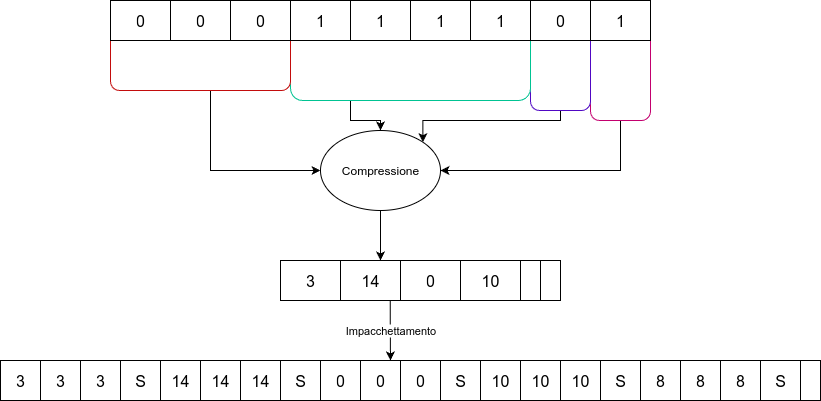
\includegraphics[width=0.75\textwidth]{immagini/run_length.png}
    \caption{Compressione ed impacchettamento mediante Algoritmo Run-Length S= Silenzio}
    \label{fig:run_length}
\end{figure}

   Nel seguente frammento  è mostrata la parte conclusiva di \textbf{bit\_output\_packer\_convert} che aggiunge il Code terminatore 8 (21 zeri) 
  ed il silenzio finale che verrà interpretato come un silenzio di 80ms dal modulo \textbf{emit\_tones}:

\begin{minted}[linenos,breaklines]{c}
for(int b = 6; b >= 0; --b){
    printf(" 8 ");
    packer->pairs[packer->pair_count++] = frequency_coder(8, role);
}
packer->pairs[packer->pair_count++] = silent;
\end{minted}

\section{Instradamento e protocollo}

Il livello superiore, il Livello Link, del protocollo è rappresentato da \textbf{protocol.c}, dove vengono gestite l’assegnazione degli identificativi, 
l’emissione di comandi e la ricezione delle risposte. \\
I messaggi, incapsulati con la sintassi \textbf{ID:\{dest\}\{OP\}k\{src\}}, come discusso nella \autoref{sec:livello_link} ed nella \autoref{subsec:registrazione}
 vengono convogliati 
all’uscita del canale appropriato tramite \textbf{send\_master}, \textbf{send\_slave} o \textbf{send\_config}.\\
 Ogni funzione di trasmissione sfrutta 
\textbf{bit\_output\_packer} ed \textbf{emit\_tones}, ma si differenzia per la portante adottata. Il frammento seguente illustra la procedura di invio
 sul canale master:

\begin{minted}[linenos,breaklines]{c}
static unsigned long send_master(const char *msg){
    log_send(msg);
    BitOutputPacker packer;
    bit_output_packer_init(&packer);
    unsigned long duration = 0;
    if(bit_output_packer_compress(&packer, msg)){
        if(bit_output_packer_convert(&packer, 0)){
            duration = estimate_send_duration(&packer);
            emit_tones(packer.pairs, packer.pair_count);
        }
    }
    bit_output_packer_free(&packer);
    return duration;
}
\end{minted}

La funzione calcola anche il tempo necessario alla trasmissione attraverso \textbf{estimate\_send\_duration},
 valore impiegato per ritardare eventuali retransmission in caso di mancato ACK. All’interno della routine \textbf{protocol\_handle\_message} 
 sono implementate le sequenze di registrazione, il meccanismo del token di trasmissione e la mappatura dei comandi provenienti dall’interfaccia esterna.\\
  Quando un nodo privo di identificativo invia una richiesta \textbf{\{REQ\}l\{xxx\}}, l’hotspot genera un ID univoco e risponde con il messaggio 
  \textbf{ID:idAssegnato\{SET\}k\{0000\}}; il nodo memorizza l’ID non volatile e conferma con \textbf{\{OK\}}. Le stesse routine gestiscono anche 
  le operazioni \textbf{ABORT} e \textbf{MOVEMENT}, delegando al modulo \textbf{movement\_sensor} l’effettiva lettura del sensore PIR.

  \section{Sensore di movimento}

  Infine per mostrare come il protocollo possa essere esteso con funzionalità pratiche, è stato sviluppato il modulo \textbf{movement\_sensor}, che non appartiene al
  protocollo in senso stretto, ma è la prima applicazione del \textbf{Livello Applicativo}. 
  La routine \textbf{movement\_sensor\_detect} attiva il sensore PIR per un intervallo prefissato e restituisce \textbf{true} o \textbf{false} 
  a seconda della rilevazione. Alla ricezione del comando \textbf{MOVEMENT:ON\_xxx}, il protocollo esegue la chiamata e risponde con \textbf{MOVEMENT:YES} 
  o \textbf{MOVEMENT:NO}, questo per offrire all'utilizzatore del sistema un'astrazione sulla quale sfruttando le potezialità di
  un browser web, si può costruire un'interfaccia utente.